Figure~\ref{fig:newplan}(a)-(e) shows the savings from scheduling each type of load in isolation for increasing values of $\alpha$. For these experiments, we chose the consumer-specific target to be equal to the home's average power.    In this case, for each load, we evaluate it using the ``reasonable" values from Figure~\ref{fig:oldplan}(f):  a two-hour duty cycle for the shiftable loads, four hours for the delay time, and 2x for the stretch factor.  For storage and selling, we use a 10kWh battery capacity and our solar energy harvesting trace scaled at 1x.  Our results show that, in each case, the savings for modest values of $\alpha$, such as 3, are higher than for the TOU/RTP plans.  

For example, Figure~\ref{fig:newplan}(a) shows that the savings from shifting loads is 18\% for $\alpha=3$, while in Figure~\ref{fig:oldplan}(a) it is 4-7\%.  Likewise, Figure~\ref{fig:newplan}(b) shows that the savings from sliding loads is 13\% for $\alpha=3$, while in Figure~\ref{fig:oldplan}(b) it is $\sim$6\%.  Stretching and storing power also show greater benefits.  Flat-power pricing is particularly attractive for storage, since it takes much less storage capacity to flatten a home's demand than to shift all of its demand to the low-price period.  We explore this aspect of scheduling storage in recent work~\cite{peakcharge}, although using a peak-based pricing plan based on a home's absolute peak.  As we mention, one difficulty with peak-based pricing is the difficulty in predicting when the absolute peak will occur.  For scheduling storage, flat-power pricing eliminates this difficulty, while preserving the incentive to flatten demand, making it more conducive to algorithmic optimization.  Interestingly, solar harvesting offers roughly the same benefit as with the TOU/RTP plans ($\sim$50\%) at 1x scale.  The reason is that with TOU/RTP plans, solar plans produce energy near the optimal time to minimize costs, i.e., during peak periods. In addition, for increasing values of $\alpha$, solar energy actually sees decreasing relative savings with flat-power pricing.  Since we choose the target to be equal to the home's average power, the increasing amount of solar energy lowers the consumer-specific target resulting in higher prices due to more electricity usage being above the target.  This dynamic demonstrates that the consumer-specific target should be independent of a home's renewable energy generation.  

Finally, Figure~\ref{fig:newplan}(f) shows the savings from the same combined load scheduling as in Figure~\ref{fig:oldplan}(f) for increasing values of $\alpha$.  Without any energy storage or renewable energy, the savings are 30\% for an $\alpha=3$ and up to 40\% with higher $\alpha$ values, compared to the 11\% and 20\% savings in the TOU and RTP cases, respectively.  In addition, if we add in 10kWh of energy storage and 1x of solar generation, the savings are 77\% for $\alpha=3$, compared with 40\% and 25\% when adding energy storage and 1x of solar generation in the TOU and RTP cases.  The results show that flat-power pricing offers consumers a greater incentive in all cases to schedule loads than existing TOU/RTP plans, enabling utilities to control the incentive by raising or lowering the $\alpha$ parameter.  



%Flat-power pricing is also attractive for storage, since it requires less storage capacity to flatten demand than to transfer large amounts of demand to low-price periods.  


%Interestingly, 


































%% \begin{figure*}[t]
%% \centering
%% \begin{tabular}{ccc}
%% \includegraphics[width=0.30\textwidth]{graphs/dong/evaluation/sw_mean.pdf} &
%% \includegraphics[width=0.30\textwidth]{graphs/dong/evaluation/sw_range.pdf} &
%% \includegraphics[width=0.30\textwidth]{graphs/dong/evaluation/sw_sd.pdf}\\ 
%% (a) Mean Power & (b) Range Power & (c) Standard Derivation
%% \end{tabular}
%% \vspace{0.2cm}
%% \caption{The mean power (a), range power (b), and Standard Derivation (c) over the two typical weeks of spring and summer for Home-A.}
%% \label{fig:background-metrics}
%% \vspace{-0.4cm}
%% \end{figure*}
%
%
%
%% \begin{figure}[t]
%% \centering
%% \includegraphics[width=0.45\textwidth]{graphs/dong/evaluation/sw_range.pdf}
%% \caption{The mean power (a), range power (b), and Standard Derivation (c) over the two typical weeks of spring and summer for Home-A.}
%% \label{fig:example}
%% \end{figure}
%
%% Figure~\ref{fig:example} shows blah blah blah
%
%%
%%\begin{figure*}[t]
%%\centering
%%\begin{tabular}{ccc}
%%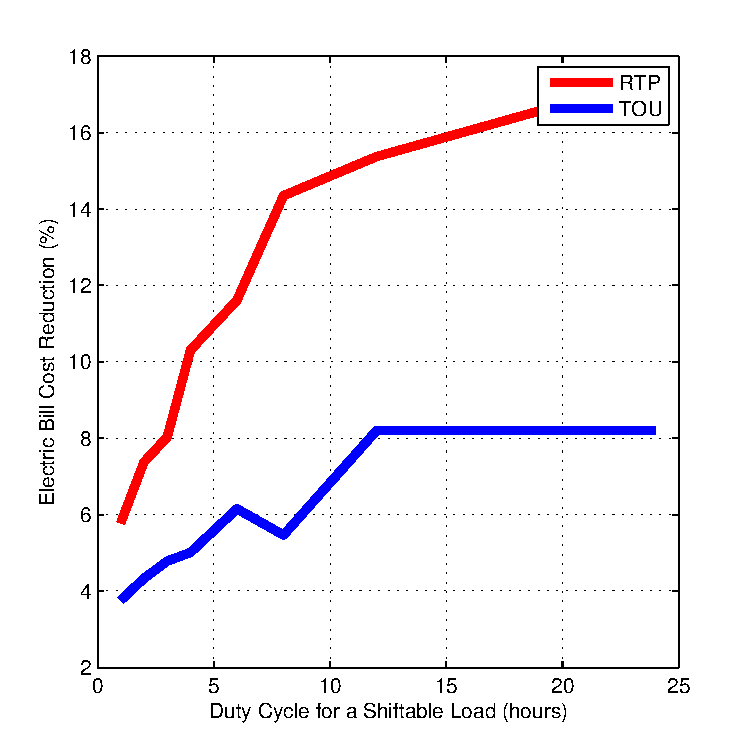
\includegraphics[width=0.33\textwidth]{graphs/shift/shiftBenefitCombined.pdf} &
%%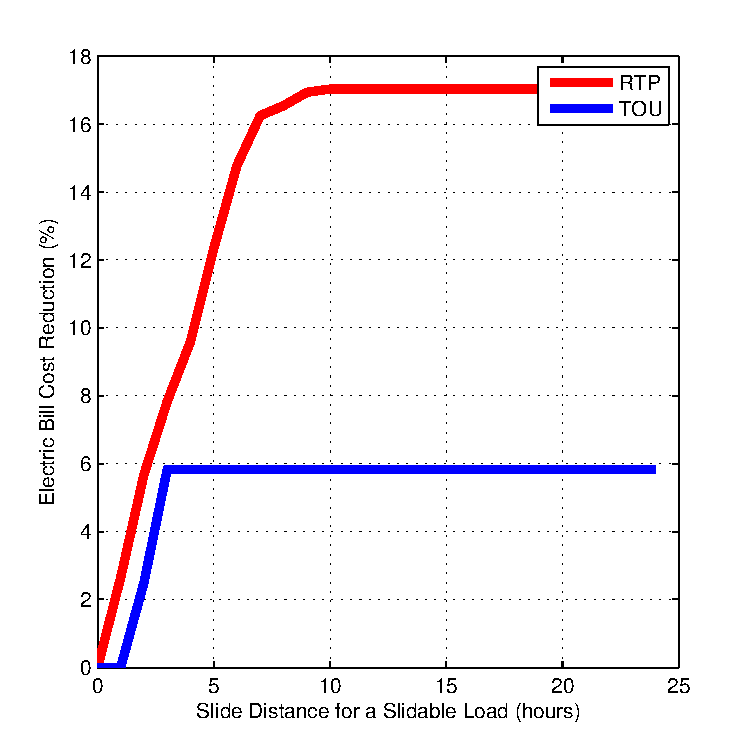
\includegraphics[width=0.33\textwidth]{graphs/slide/slideBenefitCombined.pdf} &
%%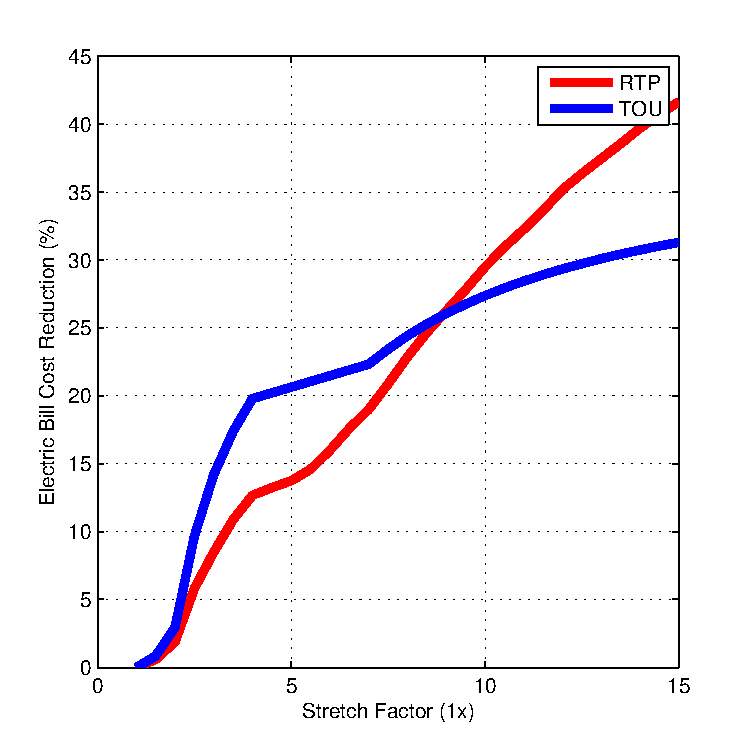
\includegraphics[width=0.33\textwidth]{graphs/stretch/stretchBenefitCombined.pdf}\\
%%(a) Shift & (b) Slide & (c) Stretch\\
%%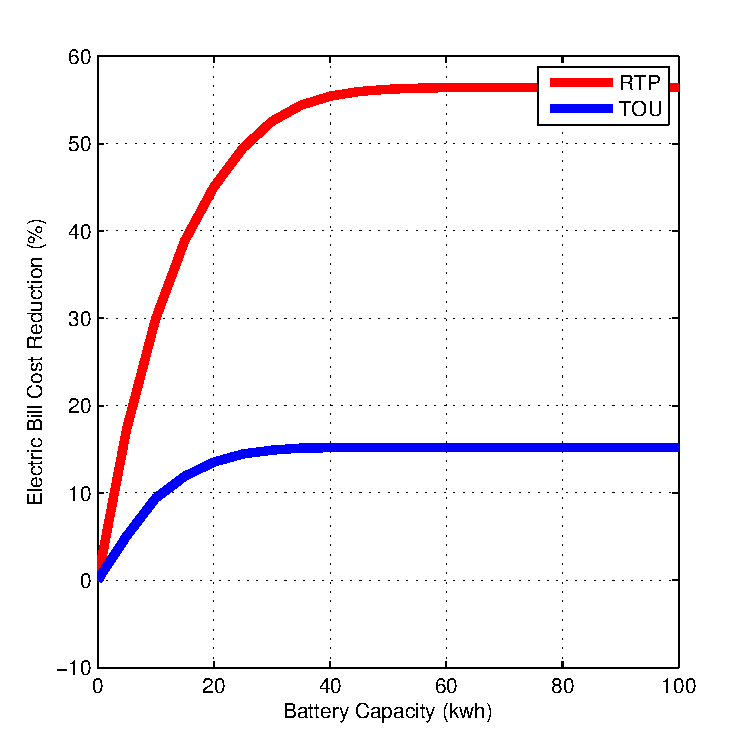
\includegraphics[width=0.33\textwidth]{graphs/store/storeBenefitCombined.pdf} &
%%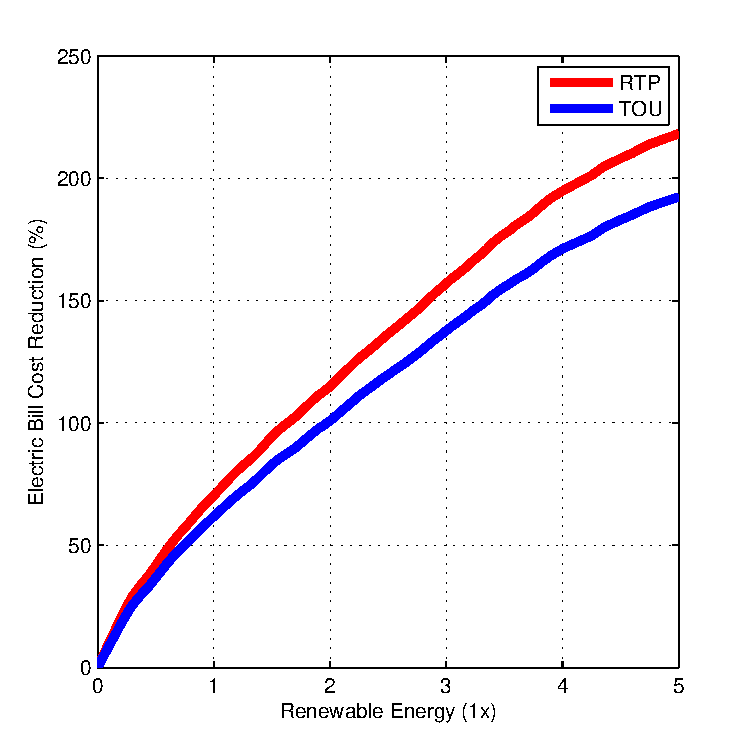
\includegraphics[width=0.33\textwidth]{graphs/sell/sellBenefitCombined.pdf} &
%%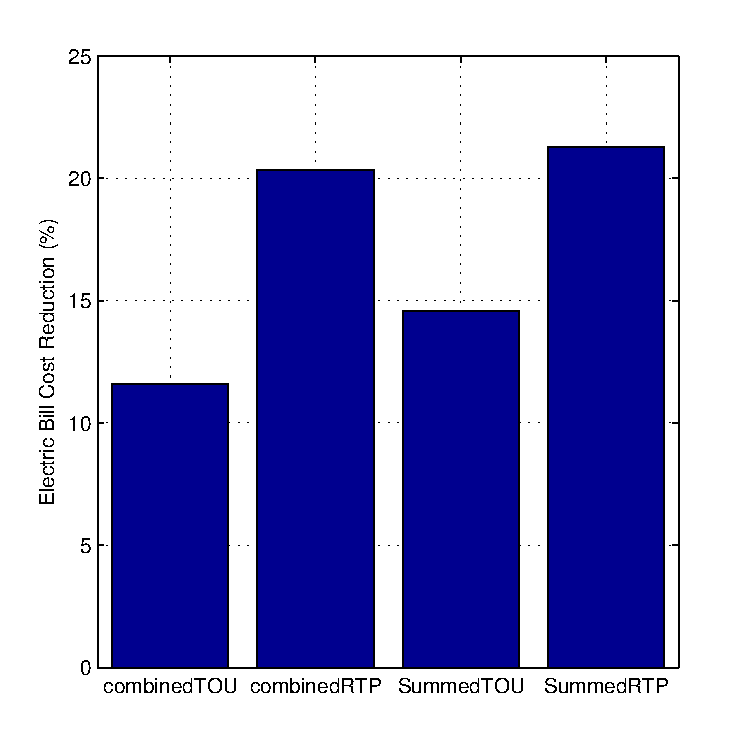
\includegraphics[width=0.33\textwidth]{graphs/combined/combinedBarGraph.pdf}\\
%%(d) Store & (e) Slide & (f) Combined\\
%%\end{tabular}
%%\vspace{0.2cm}
%%\caption{Cost  from scheduling shiftable, slidable, and stretchable loads as scheduling freedom increases.}
%%\label{fig:oldplan}
%%\vspace{-0.4cm}
%%\end{figure*}
%%
%%\begin{figure*}[t]
%%\centering
%%\begin{tabular}{cc}
%%(a) Store & (b) Sell
%%\end{tabular}
%%\vspace{0.2cm}
%%\caption{Cost savings from using energy storage and net metering, as capacity and renewable generation increases.}
%%\label{fig:isolation2}
%%\vspace{-0.4cm}
%%\end{figure*}
%
%\begin{figure*}[t]
%\centering
%\begin{tabular}{ccc}
%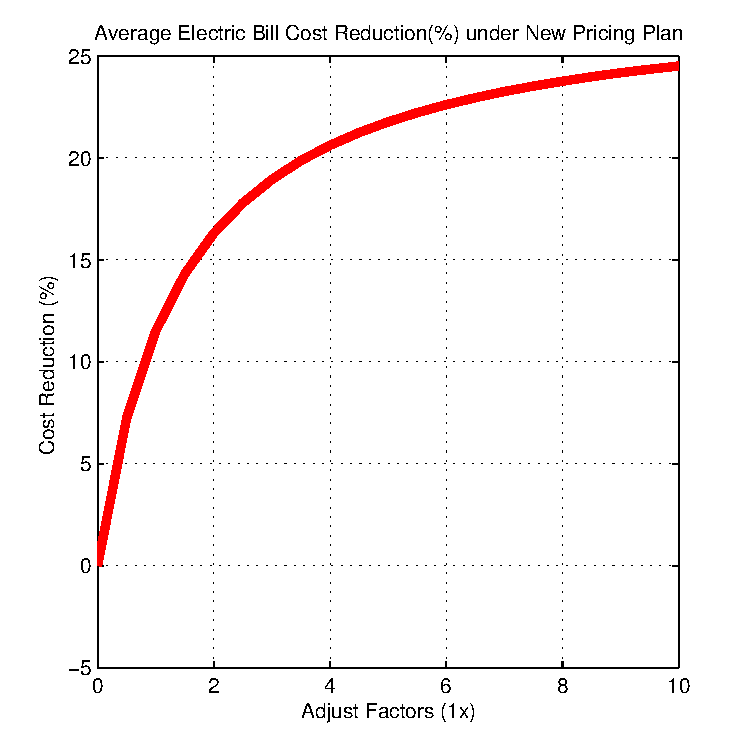
\includegraphics[width=0.33\textwidth]{graphs/shift/shiftBenefitNew.pdf} &
%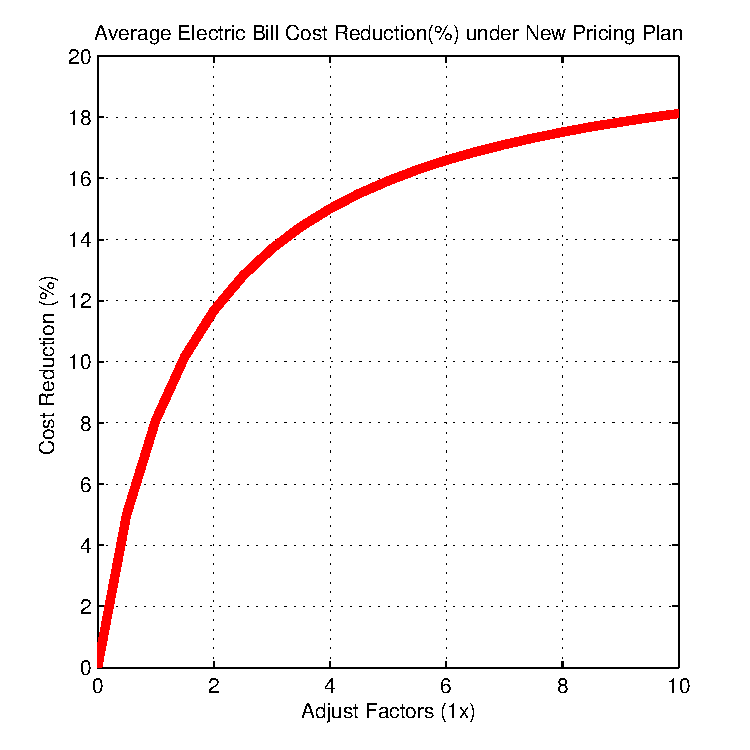
\includegraphics[width=0.33\textwidth]{graphs/slide/slideBenefitNew.pdf} &
%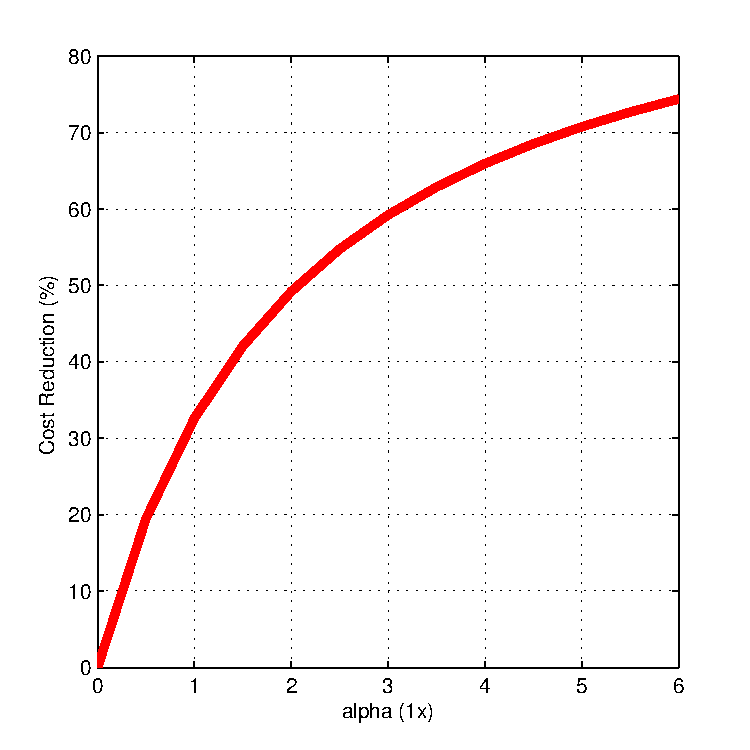
\includegraphics[width=0.33\textwidth]{graphs/stretch/stretchBenefitNew.pdf}\\
%(a) Shift & (b) Slide & (c) Stretch\\
%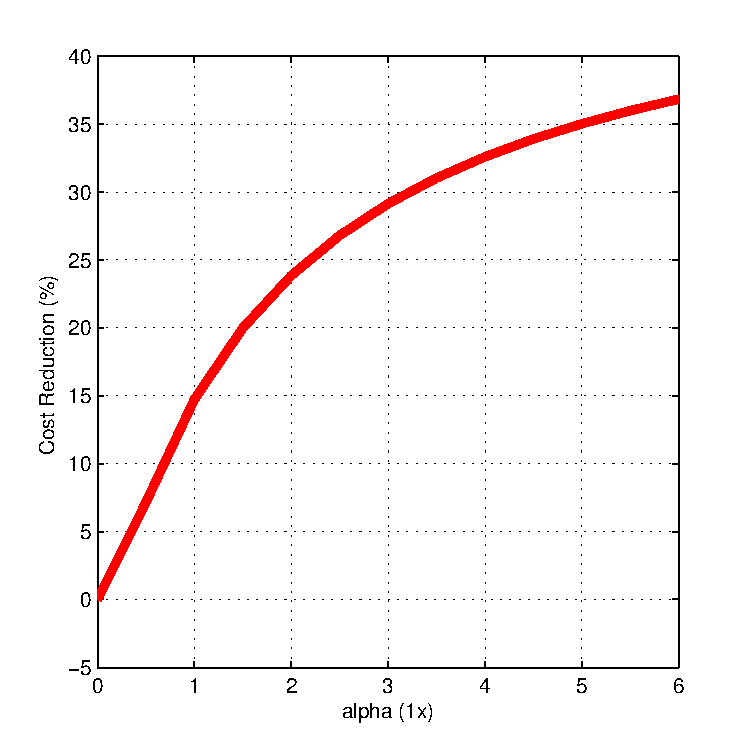
\includegraphics[width=0.33\textwidth]{graphs/store/storageBenefitNew.pdf} &
%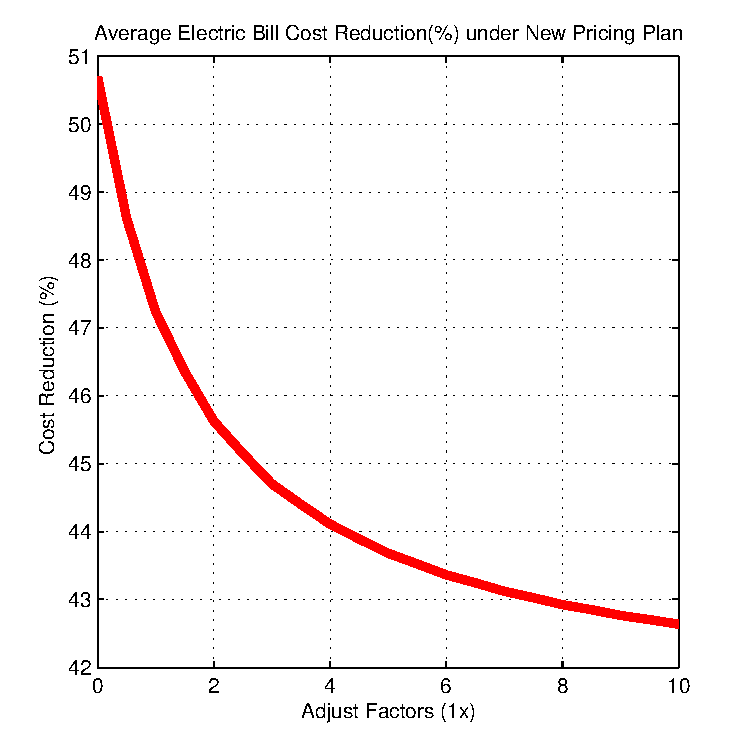
\includegraphics[width=0.33\textwidth]{graphs/sell/sellBenefitNew.pdf} &
%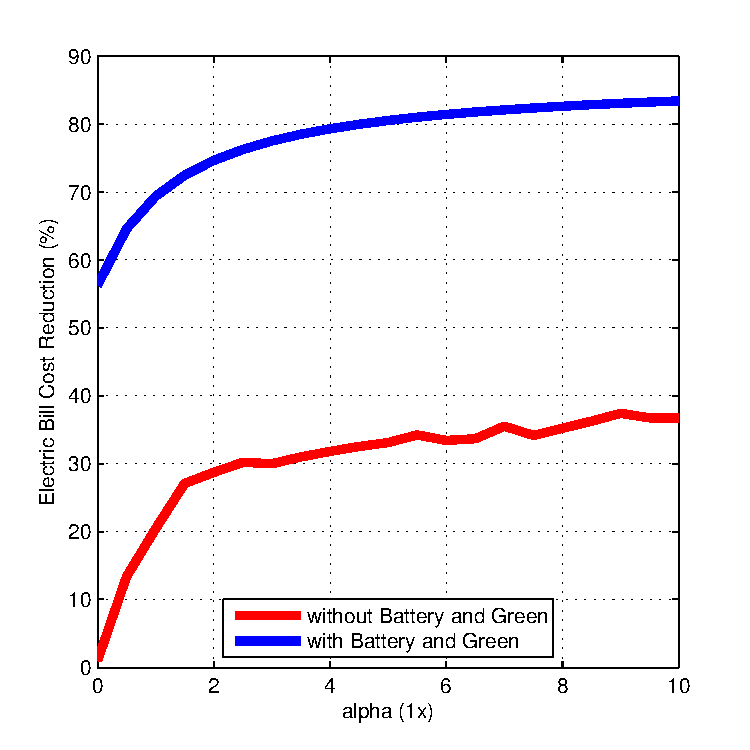
\includegraphics[width=0.33\textwidth]{graphs/combined/CombinedNew.pdf}\\
%(d) Store & (e) Sell & (f) Combined\\
%\end{tabular}
%\vspace{0.2cm}
%\caption{Cost savings from optimizing each degree of scheduling freedom(shifting, sliding, stretching, storing, selling and in combination) under Flat-power pricing within reasonable limits.}
%\label{fig:newplan}
%\vspace{-0.4cm}
%\end{figure*}
%
%
%\subsection{Assumptions}
%The following data and assumptions are used for all the simulations:
%\newline 1. The energy consumption dataset was from the smart house\cite{smart-star}, from July 1st, 2012 to Aug. 30th, 2012, for 61 days in total.
%\newline 2. We assume that our system can behave like an oracle, in other words, it knows next day’s power pattern(based on the energy consumption dataset) and solar availability during that day. 
%\newline 3. RTP, TOU, and Solar(Green) energy used in the simulation are the same for all 61 days. RTP and TOU pricing plan are taken from Figure 1. As for the solar energy, we assume it is a sunny day with the most solar available from 11am to 3pm.
%\newline 4. The Flat-power pricing plan, was generated based on the TOU plan. We first calculated the average TOU rate as well as the average power for one time step. Then we set the real rate above the average if the real power usage for one specific time step is higher than the average power, set the rate the same as the average rate otherwise. 
%\newline 5. The shiftable load used here is the Central AC system with a energy usage of 13 kwh one day. The running time during each duty cycle is set as the one third time of the duty cycle. And the slidable as well as the stretchable load is the dishwasher with a static profile as follows:  e =[ 0 1 0 0 1 0], 0 means it is non elastic phase and 1 otherwise. Power Per Phase = [ 0.25 1 0.25 0.5 1 0.25] in kw, duration Per Phase = [0.25 0.25 0.75 0.25 0.25 0.25] in hours.
%\newline 6. For each simulation, we assume the original bill is based on the worst case situation. For example, the worst case situation for slideable and stretchable loads are that the start running time is always in the time step with the highest rate. 
%
%\subsection{Discussion}
%%For each simulation graph in Figure 2, the cost savings under RTP is more than that under TOU, which simply indicates that the less fixed pricing plan, the more benefit one can get in terms of cost savings using our optimizing scheduling techniques.
%
%\\Figure 2(a) shows that increasing the duty cycle would actually increase the cost savings benefit. For example, if the shiftable load's duty cycle is just one hour, with a running time of 1/3 hour. We don't have much scheduling freedom, since no matter how we shift the load, the price within one time step is fixed, thus the total cost would be the same. On the other hand, if the duty cycle is a few hours, then we can turn off the load during high-rate periods, and turn it on during low-rate periods, as long as the total energy required to run the load remains the same.
%
%\\Figure 2(b) shows that after a specific slide distance, both the RTP and TOU pricing plan would remain a same cost benefit. This is because at that point, the rate hits the lowest value. Therefore, even if the slide distance keeps increasing, the scheduling algorithm would still pick that lowest time point to run the load.
%
%\\Figure 2(d) also shows that after a battery capacity points, the cost savings goes to saturation. This is because even if the battery capacity increases further, the total energy for the entire house one day is already lower than the capacity, thus the benefit would not go up with more capacity. 
%
%\\Figure 2(f) uses a set of parameters as follows: AC energy used one day is 13 kwh, duty cycle 2 hours, running time at each duty cycle is 2/3 hours; Dishwasher's elasticity profile is same as in assumption 5, but the slide distance is 4 hours, the stretch factor is 2. The battery capacity is 10 kwh. It shows that the combined benefit would be lower than the individual benefit summed up. This is because when combining all the scheduling together, there are additional constraints that must be satisfied. For example, We cannot use the batteries and do net metering at the same time.
%
%\\Figure 4 shows the cost savings under the Flat-power pricing plan, using the same parameters as in Figure 2(f).From the graphs we can see that with a certain alpha, there would be more savings than TOU; with a even higher alpha, it would ultimately go beyond the savings of RTP. For example, in Figure 4(f), if without battery and green energy source, an alpha of 1 can bring more cost savings(20\%) than combined TOU(13\%), and an alpha of 1.5 can bring more savings(25\%) than combined RTP(21\%).   
%
%\\Figure 4((a)-(d)) shows that the cost benefit would go up as the alpha increases, but with a smaller slope. The smaller slope results from the fact that the shiftable, slidable and the stretchable loads are the smaller part of the entire loads. Although these loads can be turned on and off to decrease the cost, but as the alpha increases the total bill cost would also go up, the more the total bill would be, the more dominantly the fixed part of the entire loads would take control.
%
%\\Notice that Figure 4(e)  actually goes down as the alpha increases. Based on the fact that the amount of solar energy is fixed for each time step, and 0 amount during the night time, the solar energy cannot cause the load to move to a different time step, or to be stretched out so that part of the load can run in a different time step. Thus, with the alpha increases, the total original bill would also go up, and all of the loads cannot be moved to a different time step with lower rates, the actual cost savings would go down. As for the storing case(Figure 4(d)), essentially the battery is charged using grid power during low-rate time periods, and discharged during high-rate periods, therefore it can also be treated as moving the loads to a different time step. 




